%%% untb_genomes.tex --- 

\section{Background}

Whatever the environment, terrestrial or aquatic, temperate or tropical it is universal the case that some species are very abundant, others are relatively common, and the majority, rare. What mechanisms control this uneven distribution of species abundance in ecological communities?

Species diversity and their relative abundance have always intriguing ecologists \cite{McGill2007}. Roughly speaking, ecological models of species abundance are of two kinds: descriptive (statistical-based) or mechanistic (niche-based or neutrals). While many mechanistic approaches assume niche differences as the main cause driving community composition, neutral models consider niche differences among species irrelevant \cite{Margurran2004}. The unified neutral theory of biodiversity (UNTB) \cite{Hubbell2001,Rosindell2011} is a neutral-stochastic theory originally inspired in neutral population genetic models \cite{Kimura1985,Wright1931}. UNTB assumes interactions among trophically similar species equivalent on an individual ''per capita'' basis. This provocative assumption means that these individuals, regardless of the species, appear to be controlled by similar birth, death, dispersal, and speciation rates. Since each species follows a random walk, biodiversity composition emerges regardless of specific species differences in the community. The fundamental biodiversity parameter ($\theta$), analogous to $4N\mu$­ of population genetics, governs species richness in spatial and temporal scale. Neutral theory is thus a useful null model against to test alternative biological hypotheses of relative species abundance distribution \cite{Volkov2003,Alonso2006}.

Likewise ecological communities, eukaryotes genomes contain a variable number of more or less abundant elements of different genetic classes: transposon-derived elements, satellite repetitive sequences, segmental duplications, and their less abundant functional sequences such as RNA or genes. Here, for simplicity we talk of genetic elements of different classes as individuals of different species.

Dynamical ecological models of genomes were formalized and simulated \cite{Abrusan2006,Leonardo2002,LeRouzic2007}. Some complex models parallel interactions like parasitism, competition and cooperation between different families of transposable elements (TEs). However, ideal models of genomics would consider not only TEs, but also all diversity of genetic elements populating eukaryote genomes: satellites sequences, DNA-transposons, LTR-retrotransposons, LINES, SINES, mi-RNA, rRNA, tRNA, genes, and pseudogenes among the many functional and non-functional elements. Such model does not exist for genomes.

Here, taking advantage of the methods and models developed by ecologists we ask: is there a common pattern behind the relative abundance and diversity of genetic elements in genomes? And, in the case that such pattern exists, is it sufficient to explain together diversities of  functional and non-functional components in eukaryote genomes? To what extent abundance and diversity of genome components reflects adaptive or stochastic outcomes? Here we test the statistical adjustment of the UNTB predictions to more than 30 different eukaryote genomes.

To achieve this objective we discuss results in three different sections. First we analyze genomes and chromosomes by virtue of relative species abundance (RSA) curves, classical graphical tools used in ecology to know if genomes and chromosomes display uneven species distributions as is universally observed in ecological communities. Second we simulate the random distribution of all elements of genomes in all their chromosomes to statistically test the role of chance in chromosome design. Third, we test the statistical adjustment of the neutral ecological theory of biodiversity to the relative abundance and diversity of functional and non-functional elements of eukaryote chromosomes.

We conclude that abundances and diversity of genetic elements in most chromosomes is predicted by the stochastic dynamics of a model for which the principle of functional equivalence among elements is the primary assumption. Finally, we present a strong test to the hypothesis. If functional and non-functional genetic elements are distributed stochastically in chromosomes, their length must be predicted by demographic parameters only. Ecologists assert that effects of natural selection are dispensable to model abundance and species diversity in tropical forest \cite{Jabot2011}. Paralleling ecological communities Darwinian dynamics seems to be irrelevant to define abundance and diversity of genome components.

\section{Results}

\subsection{Genomic elements, dispersion and abundance}

Ecologists frequently use RSA curves to compare the richness, the degree of dominance, and the number of rare species in communities. The raw data used in these plots is the total number of individuals per species sampled in the ecosystem. The most interesting property of RSA curves is that species are unlabeled in the ranking order; hence ecosystems can be compared whatever the species they contain.

Taking advantage of the current automatic methods of genome annotation and string recognition, all genetic elements belonging to different functional and non-functional classes were counted to build RSA curves in genomes and chromosomes. These numbers represent censuses of genomic elements analogous to those sampled in ecosystems.

\begin{FPfigure}
\centering 
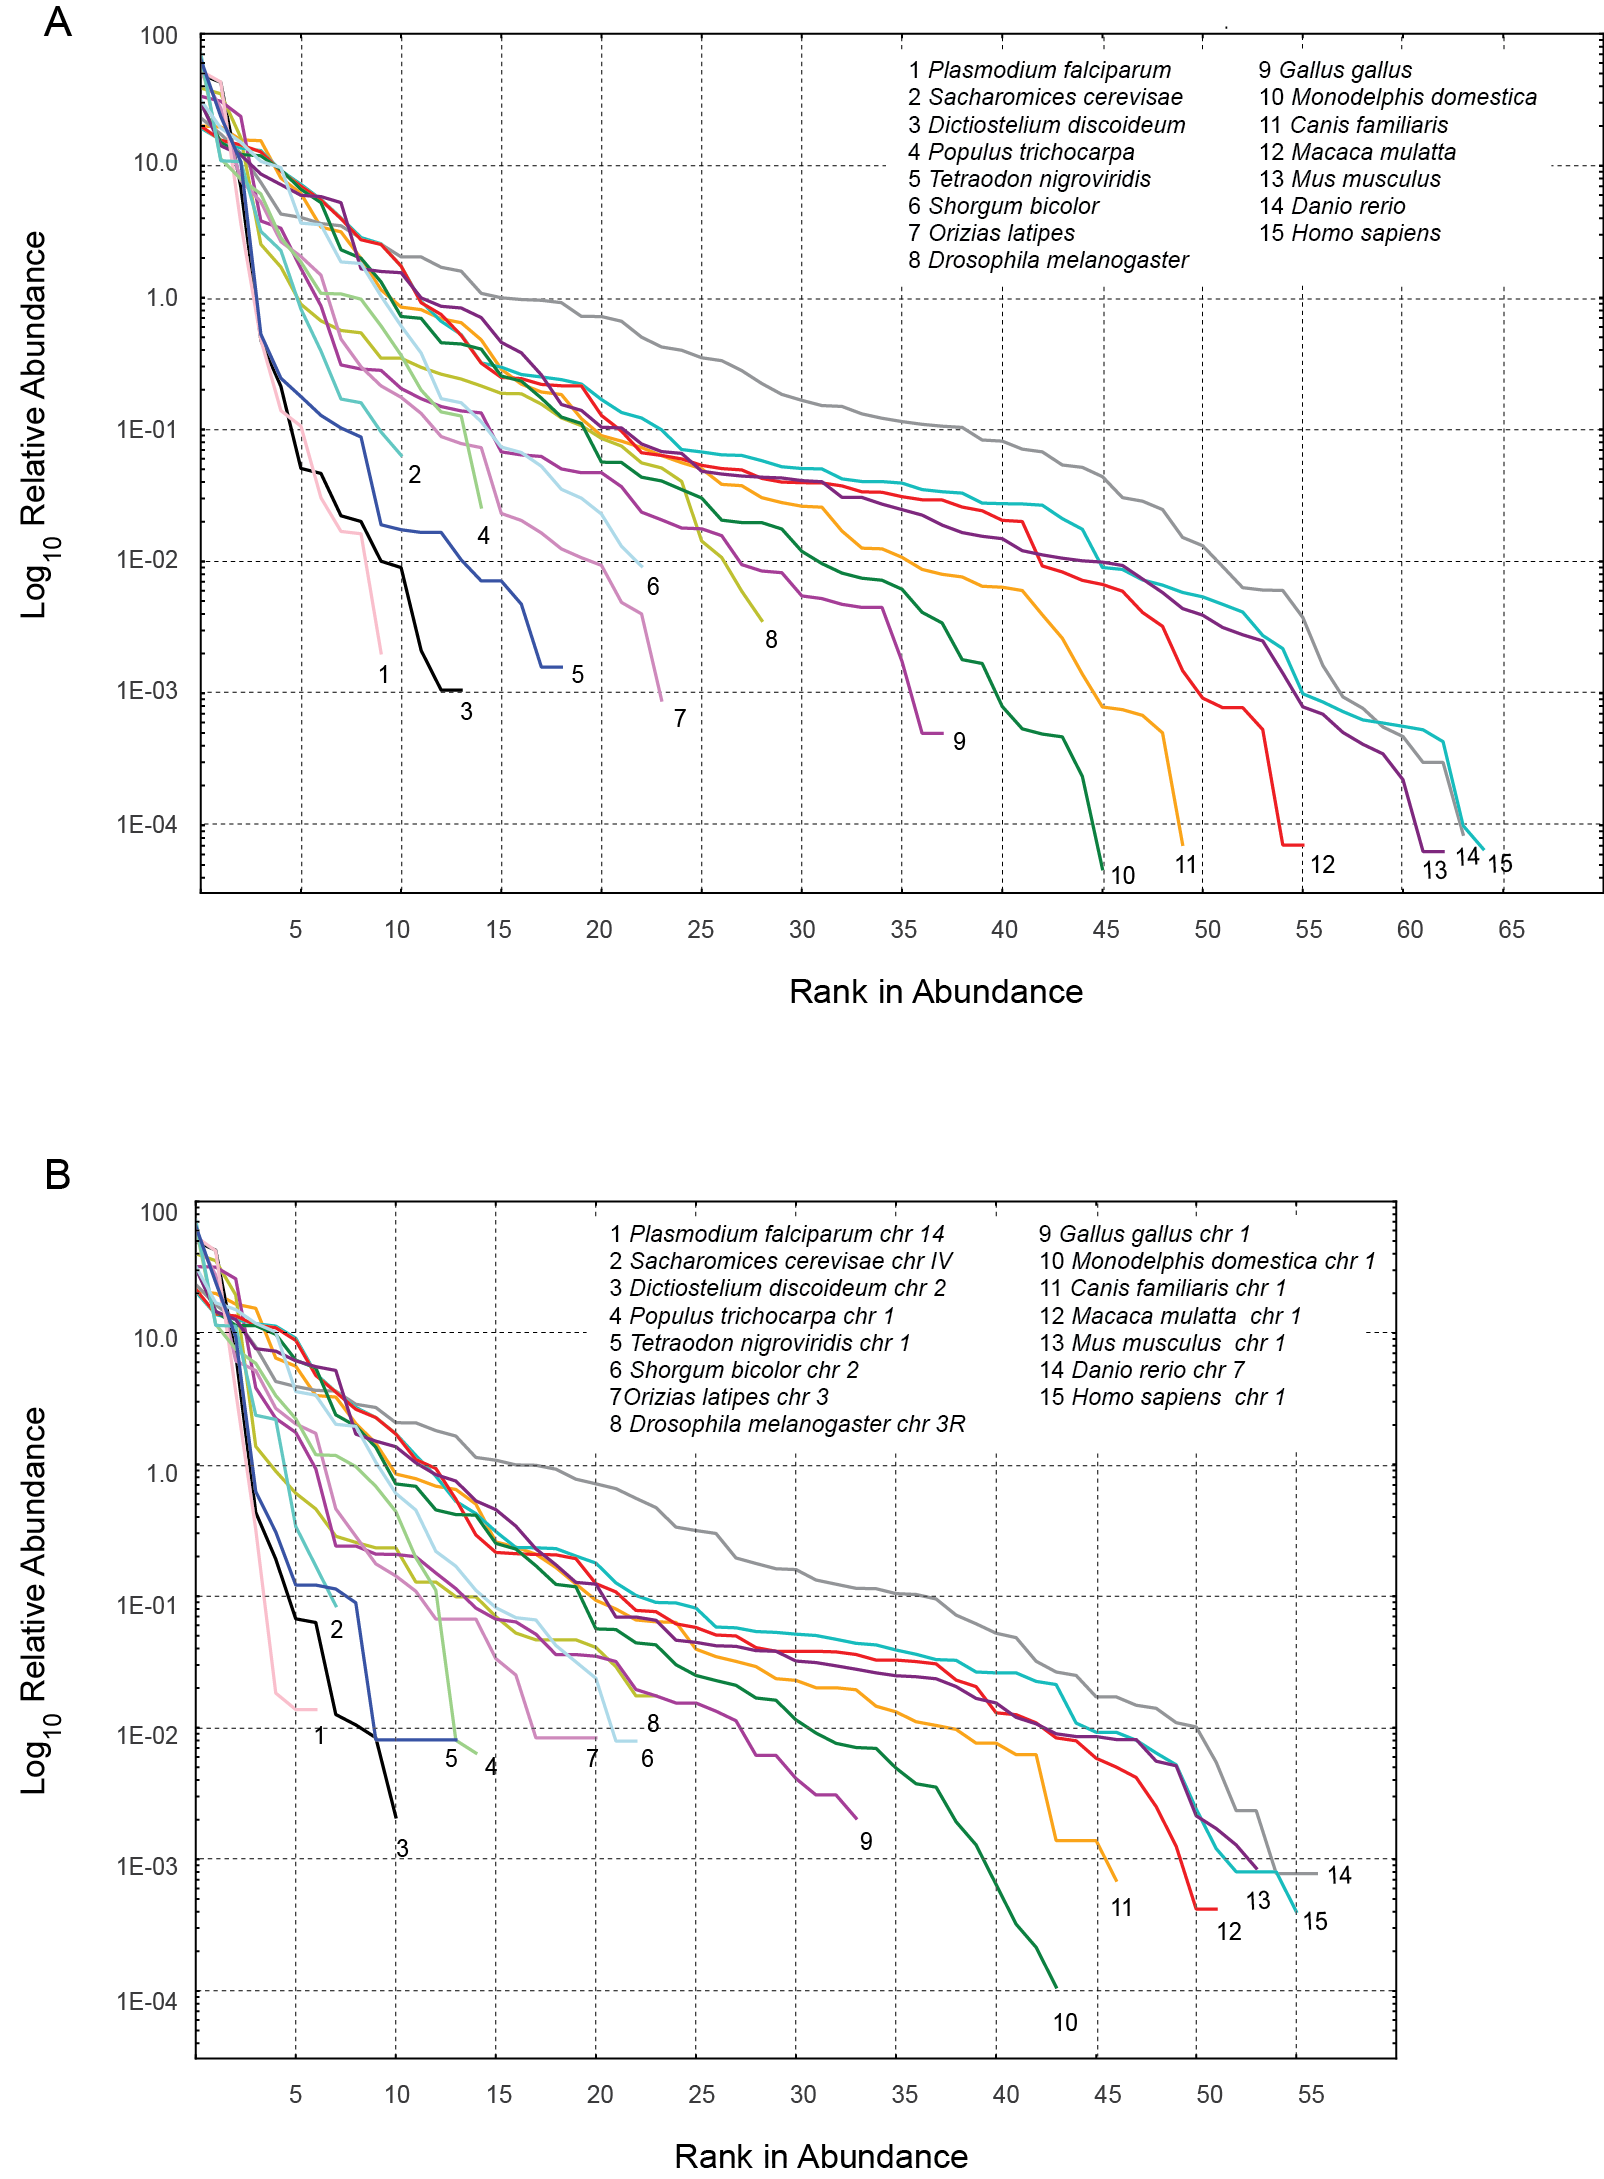
\includegraphics[width=\textwidth]{tex_source/figures/untb_genomes/SAD_genomes.png}
\caption[RSA curves.]{{\bf RSA curves.} \\ Relative species abundances for some selected genomes (A) and their corresponding largest chromosomes (B)} 
\label{fig:rsa_genomes}
\end{FPfigure}

\fref{fig:rsa_genomes}{} display RSA curves for a selected group of genomes and their largest chromosome respectively. Curves differ in many ways although two patterns are evident: 1- RSA curves of genomes and chromosomes are very similar for species, 2- all RSA curves display the universal S-shape observed in ecological environments \cite{McGill2007,Hubbell2001}. Both observations suggest a common mechanism of distribution of genetic elements in genomes and chromosomes.

\subsection{Counterbalanced species abundances in genomes}

To what extent chromosome's RSA curves represent the random distribution of the complete set of elements of the genome? To answer, we simulate the random distribution of the full set of genetic elements reported in genomes in their corresponding chromosomes. After one thousand simulations the mean expected abundance and its standard deviation were computed for all genetic classes in chromosomes. These values were used to plot random expected RSA curves for chromosomes.

Statistical tests (t-test, $FDR<0.05$) established that less than 1\% of all genetic classes in all chromosomes tested showed abundances according to their random expected distribution. This homogeneous process therefore, does not account for the observed RSA curves in chromosomes. However, another kind of arbitrary process is suggested for chromosomes if simulated and observed RSA curves are superimposed \fref{fig:rsa_chromosomes}{}.

\begin{FPfigure}
\centering 
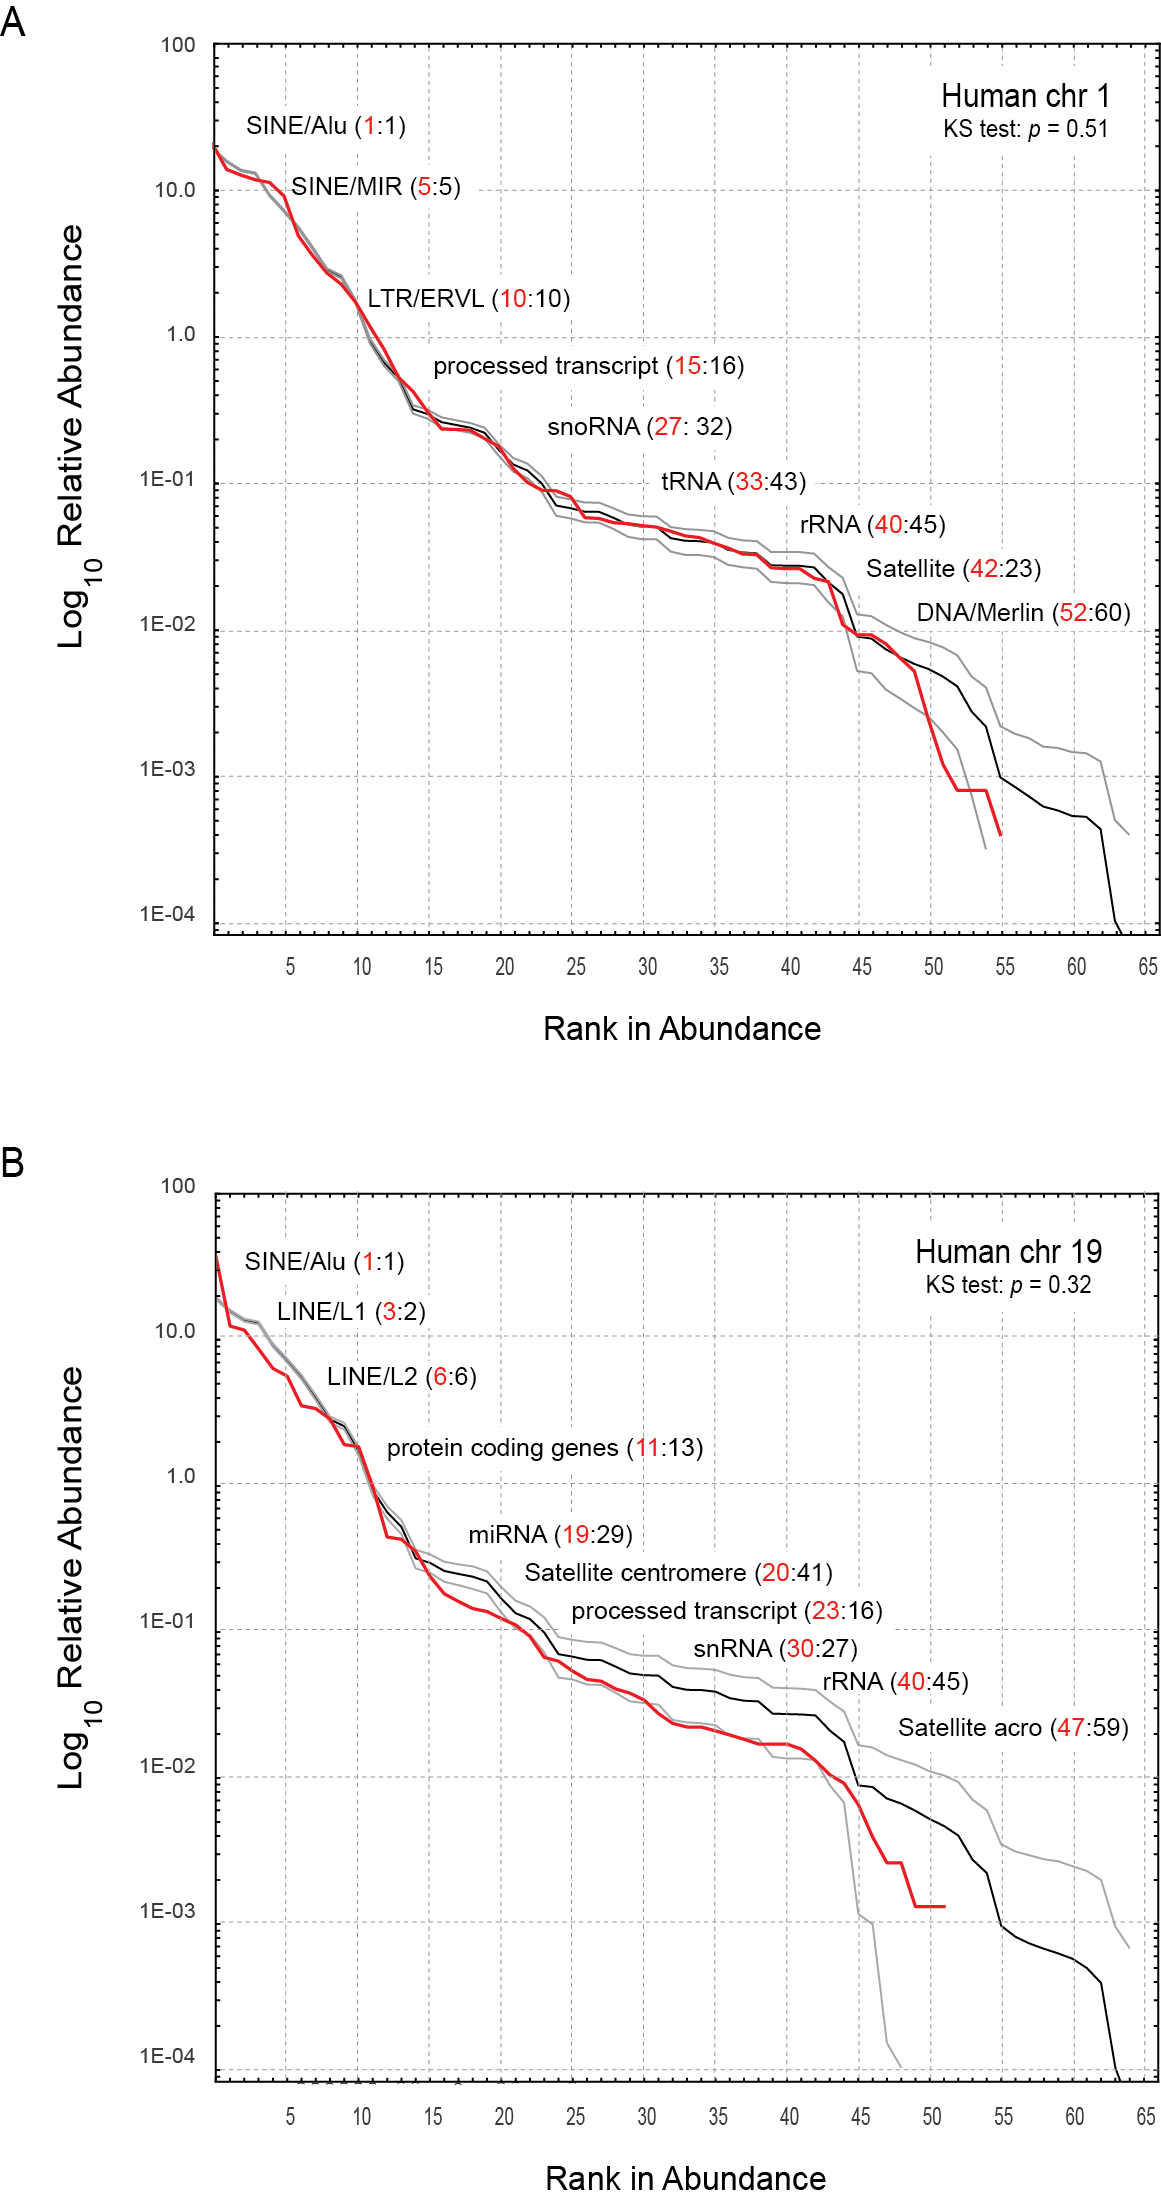
\includegraphics[height=\textheight]{tex_source/figures/untb_genomes/ra_chroms.png}
\caption[Relative species abundance curves for human chr 1 and chr 19]{{\bf Relative species abundance curves for human chr 1 (A) and chr 19 (B).} \\ Relative species abundance curves for human chr 1 (A) and chr 19 (B). Red and black lines display observed and simulated RSA curves for all functional and non-functional genetic classes in chromosomes respectively. Grey lines show two standard deviations around the mean of the simulated data. The absence of statistical differences between RSA curves is mainly due to the frequent counterbalanced changes observed in the ranking of abundances of genetic classes. Numbers in parenthesis depict the observed (red) and the expected value (black) in the ranking of abundances for few genetic classes in both chromosomes. Differences between numbers point out over and under abundances in chromosomes. Note the higher than the expected number of SINE/Alu elements in human chromosome 19 (class 1 in the ranking).} 
\label{fig:rsa_chromosomes}
\end{FPfigure}

This notable adjustment is due to the fact that genetic classes are unlabeled in the ranking order, and changes in the order of abundances are counterbalanced in chromosomes. For instance, the classes of functional tRNA and satellite elements are at position 33 and 42 of the ranking of abundances respectively in human chromosome 1 \fref{fig:rsa_chromosomes}{-A}. However, according to their random distribution the expected values in the ranking are 43 and 23 respectively. That is, tRNA and satellite elements show higher and lower abundances than the expected by random distribution. Over and under abundances of different genetic classes counterbalance each other in the same chromosome leading to an almost perfect fit between observed and expected RSA curves. We only found significant differences between observed and expected RSA curves for less than 100 of most 540 chromosomes tested (KS test, $p < 0.05$).

What is the mechanism contributing to this counterbalanced dynamics of genetic elements in eukaryote's chromosomes? Next, we test the neutral theory of biodiversity as the main explanation accounting for such events in genomes.


\subsection{Neutrality of SAD}

Similar to the kinetic theory of ideal gases in physics the neutral theory of biodiversity is a stochastic theory assuming equivalence among interacting individuals. The theory assumes that diversity in a local community of individuals is maintained by migration from the metacommunity at a constant rate ($m$). Births and deaths in the local community occur at constant rates during generation regardless the species. The metacommunity dynamics is controlled by speciation at a single constant rate ($\nu$)\cite{Rosindell2011,Alonso2006}.

For genomes, we realized that each chromosome is the physical arena where genetic elements die and are replaced by other elements of the same or different species. These genetic elements could come from the same chromosome, or from any other chromosome of the genome. We assume that each chromosome represents a local community of $J$ elements and $S$ different genetic classes (species) while the rest of chromosomes correspond to the metacommunity of size $J_M$. Thus, given the total number of functional and non-functional elements in each chromosome we optimized by maximum likelihood (ML) the neutral theory's parameters m and $\theta$ ($= 2 J_M\nu$) using Ewens and Etienne's sampling formula (\ref{eq:ewens}) (see example \fref{fig:lnl_chrom}{}).

Deviations of neutrality were detected in 33 out of 578 (5.7\%) chromosomes. However, deviations vanished at all after multiple testing correction ($FDR< 0.05$, Table). We conclude that Hubbell's neutral model fits abundance and diversity of genetic elements in all the chromosomes of the 31 eukaryotes genomes analyzed. 


\subsection{Diversity and chromosome length}

\section{Discussion}

Abundance and diversity of selfish genetic elements \cite{Doolittle1980,Orgel1980} results from millions of years of close interaction with their host, the genome. Population dynamics models dealing with transposable elements (TE) has been formalized and reviewed \cite{Charlesworth2009,Charlesworth1994,LeRouzic2005}. Transposition and excision rates, as well as host fitness impact are some of their most significant parameters. While the predicted deleterious effects of transposition have been confirmed repeatedly in Drosophila (citar...), almost a neutral accumulation of TEs is expected in mammals due to the larger genomes and smaller population size18. An important concern with these models is the explicit absence of relationships of TEs with other genetic components of the genome. 

The general transposition-selection based model predicts an adaptive equilibrium of TE abundance. However, abundances of the same TE differ between population and species (citar). 
Additionally, models c 9-11. Importantly variation between individuals was observed...\cite{Brookfield2005}

However, a former question is mandatory: Did TE's diversity and abundance features shaped by random processes in genomes \cite{Lynch2003,Venner2009}. 

Nature seems to play forest and genomes with the same dice.
Functional elements, as expected deviates expectations If functional elements are excluded from chromosomes, neutrality was rejected in a single chromosome (D. rerio chr2, p= 0.04, q= 0.36).


\section{Material Methods}

\subsection{Genomes}

Genomic sequences of 31 species from unicellular eukaryotes to mammals were used, all were extracted from previous work see Section \ref{sec:complexity-strings} and \tref{tab:genome}. The complete list of species used is: \begin{inparaenum}[\itshape 1)]
\item \textit{Gallus gallus} (Birds)
\item \textit{Taeniopygia guttata} (Birds)
\item \textit{Danio rerio} (Fishes)
\item \textit{Oryzias latipes} (Fishes)
\item \textit{Tetraodon nigroviridis} (Fishes)
\item \textit{Saccharomyces cerevisiae} (Fungi)
\item \textit{Anopheles gambiae} (Invertebrates)
\item \textit{Caenorhabditis elegans} (Invertebrates)
\item \textit{Drosophila melanogaster} (Invertebrates)
\item \textit{Tribolium castaneum} (Invertebrates)
\item \textit{Bos taurus} (Mammals)
\item \textit{Canis familiaris} (Mammals)
\item \textit{Equus caballus} (Mammals)
\item \textit{Homo sapiens} (Mammals)
\item \textit{Macaca mulatta} (Mammals)
\item \textit{Monodelphis domestica} (Mammals)
\item \textit{Mus musculus} (Mammals)
\item \textit{Pan troglodytes} (Mammals)
\item \textit{Pongo abelii} (Mammals)
\item \textit{Rattus norvegicus} (Mammals)
\item \textit{Arabidopsis lyrata} (Plants)
\item \textit{Arabidopsis thaliana} (Plants)
\item \textit{Brachypodium distachyon} (Plants)
\item \textit{Oryza sativa} (Plants)
\item \textit{Populus trichocarpa} (Plants)
\item \textit{Sorghum bicolor} (Plants)
\item \textit{Zea mays} (Plants)
\item \textit{Dictyostelium discoideum} (unicellular Eukaryotes)
\item \textit{Plasmodium falciparum} (unicellular Eukaryotes)
\item \textit{Thalassiosira pseudonana} (unicellular Eukaryotes)
and \item \textit{Ciona intestinalis} (Urochordate)
\end{inparaenum}.

\subsection{Mining of Genomic Elements}

For this study, genomic elements were divided into 2 categories, repetitive elements and functional elements.

\subsubsection{Repetitive Elements}

Repetitive elements were retrieved using RepeatMasker \cite{Smit2010} with default parameters on whole chromosome sequences.

An example of summary file given by RepeatMasker is shown in Appendix \ref{cha:repe-summ-outp}. The definition of \textit{species}, in the context of genomic elements, was given by the class of repeats (following RepeatMasker nomenclature), subclasses were generally too rare. Here is a listing of the hierarchy of main classes and subclasses annotated by the software:
\begin{itemize}
\item Transposable Element
  \begin{itemize}
  \item DNA transposon:
    \begin{inparaenum}[\itshape 1-]
    \item Mariner/Tc1
    \item hAT
    \item MuDR
    \item EnSpm
    \item piggyBac
    \item P
    \item Merlin
    \item Harbinger
    \item Transib
    \item Novosib
    \item Mirage
    \item Helitron
    \item Polinton
    \item Rehavkus
    \item Kolobok
    \item ISL2EU
    \item Chapaev
    \item Crypton
    \item Sola
    \item Zator
    \item Ginger1
    \item Ginger2/TDD
    \item Academ 
    \end{inparaenum}
  \item LTR Retrotransposon:
    \begin{inparaenum}[\itshape 1-]
    \item Gypsy
    \item Copia
    \item BEL
    \item DIRS 
    \end{inparaenum}
  \item Endogenous Retrovirus:
    \begin{inparaenum}[\itshape 1-]
    \item ERV1
    \item ERV2
    \item ERV3
    \item Lentivirus 
    \end{inparaenum}
  \item Non-LTR Retrotransposon:
    \begin{inparaenum}[\itshape 1-]
    \item SINE:
      \begin{inparaenum}[\itshape a.]
      \item SINE1/7SL
      \item SINE2/tRNA
      \item SINE3/5S
      \item SINE4 
      \end{inparaenum}
    \item CRE
    \item NeSL
    \item R4
    \item R2
    \item L1
    \item RTE
    \item I
    \item Jockey
    \item CR1
    \item Rex1
    \item RandI
    \item Penelope
    \item Tx1
    \item RTEX
    \item Crack
    \item Nimb
    \item Proto1
    \item Proto2
    \item RTETP
    \item Hero
    \item L2
    \item Tad1
    \item Loa
    \item Ingi
    \item Outcast
    \item R1
    \item Daphne
    \item L2A
    \item L2B
    \item Ambal
    \item Vingi
    \item Kiri 
    \end{inparaenum}
  \end{itemize}
\item Simple Repeat
  \begin{itemize}
  \item Satellite:
    \begin{inparaenum}[\itshape 1-]
    \item SAT
    \item MSAT 
    \end{inparaenum}
  \end{itemize}
\item Pseudogene
  \begin{itemize}
  \item rRNA
  \item tRNA
  \item snRNA 
  \end{itemize}
\item Integrated Virus
  \begin{itemize}
  \item DNA Virus
  \item Caulimoviridae 
  \end{itemize}
\end{itemize}

\subsubsection{Functional Elements}

Functional elements correspond to the biotype category of the genes according to Ensembl \cite{Flicek2011} nomenclature. They were retrieved using the Biomart API \cite{Kinsella2011}. The non-redundant list of function elements across all species was:

\begin{inparaenum}[\itshape 1-]
  \item IG C
  \item IG D
  \item IG J
  \item IG V
  \item IG Z
  \item MRP RNA
  \item RNase MRP RNA
  \item RNase P RNA
  \item SRP RNA
  \item TR C
  \item TR J
  \item TR V
  \item class II RNA
  \item class I RNA
  \item lincRNA
  \item miRNA
  \item misc RNA
  \item ncRNA
  \item processed transcript
  \item protein coding
  \item rRNA
  \item retrotransposed
  \item snRNA
  \item snlRNA
  \item snoRNA
  \item tRNA
  and \item transposable element
\end{inparaenum}

Note that pseudogenes were removed from that list in order to keep the functional aspect of this family of genomic elements.

\subsection{Ecolopy}

Several packages or programs were already developed in order to deal with species abundances data, implementing statistical functions in order to fit data in ecological models and even able to test for neutrality \cite{Jabot2011,Etienne2007,Hankin2007}. However none of those programs were able to deal with genomic data, with abundances in the order of the million of individuals specially in the case of Etienne's model where computation of $K(D,A)$ uses stirling numbers (see Section \ref{sec:etienne-model}, equation \ref{eq:kda}). In order to adapt the algorithm to genomic dataset we developed the \textit{Ecolopy} package, that, as a main point, uses the GMP \cite{Granlund2000} and MPFR \cite{Fousse2007} libraries through GMPY biding \cite{Martelli2007}. Other improvements specific to Ecolopy, and needed for dealing with genomic dataset where done.

Ecolopy is entirely written in Python \cite{VanRossum1991}, a programming language that offers a strong support for integration with other languages and tools, and whose popularity is raising among the bioinformatics community \cite{Bassi2007}. Ecolopy is still a fully ripened package, but it was designed to provide a scalable program architecture.

\subsubsection{Ecological models}

\paragraph{Ewens} 
\label{sec:ewens-model}

Ewens sampling formula \cite{Ewens1972} (\ref{eq:ewens}) was originally designed in order to describe the number of different alleles expected to be observed in a given sample. However Tavar\'e and Ewens suggested that the formula could be applied to ecology \cite{Tavari1997} and Hubbell finally proposed a model defining the Fundamental Biodiversity parameter $\theta$ (\ref{eq:theta}) given the speciation rate $\nu$ and $J_M$ the size of the metacommunity \cite{Hubbell2001}.

\begin{equation} \label{eq:theta}
\theta = 2J_M\nu
\end{equation}

By defining $\theta$ it is possible to apply directly Ewens Sampling formula (\ref{eq:ewens}) and to compute its likelihood given a community (\ref{eq:ewens_lnl}).

\begin{equation} \label{eq:ewens}
Pr\{S,n1,n2,\ldots,n_S|\theta\} = \frac{J_M!\theta^S}{1^{\phi1} 2^{\phi2} \cdots J_M^{\phi J_M} \phi_1! \phi_2! \cdots \phi_{J_M}! \prod_{k=1}^{J_M} (\theta + k - 1)}
\end{equation}

Here $n_i$ corresponds to the abundance of species $i$ and $\phi_a$ the number of species with abundance $a$.

\begin{equation} \label{eq:ewens_lnl}
\mathcal{L} = \frac{\theta^S}{\prod_{k=1}^{J_M} (\theta + k - 1)}
\end{equation}

Given the sampling formula (\ref{eq:ewens}) Ecolopy is able to generate random neutral species abundances distributions given a sample size $J$ and a value of $\theta$. The number of species generated is free according to the formula but can be fixed by keeping only those random abundances generated with the desired number of species. The likelihood function (\ref{eq:ewens_lnl}) is also integrated in the program, and used for optimization of $\theta$ parameter (see section \ref{sec:model-optimization}).

\paragraph{Etienne}
\label{sec:etienne-model}

The main problem with Hubbell's model using Ewens sampling formula is the assumption that immigration is unlimited ($m=1$). However a new sampling formula was presented recently \cite{Etienne2005} including cases where $m<1$, taking into account the number of immigrants $I$ depending on the sample size $J$:

\begin{equation} \label{eq:m}
m = \frac{I}{I+J-1}
\end{equation}

Given this Etienne's sampling formula is postulated as:

\begin{equation} \label{eq:etienne}
P[D|\theta,m,J] = \frac{J!}{\prod_{i=1}^Sn_i \prod_{j=1}^J\phi_J!} \frac{\theta^S}{(I)_J} \sum_{A=S}^JK(D,A) \frac{I^A}{(\theta)_A}
\end{equation}

with $K(D,A)$ as:

\begin{equation} \label{eq:kda}
K(D,A) := \sum_{\{a_1,\ldots,a_s|\sum_{i=1}^Sa_i=A\}}\prod_{i=1}^S\frac{\bar{s}(n_i,a_i)\bar{s}(a_i,1)}{\bar{s}(n_i,1)}
\end{equation}

Calculation of stirling numbers here are the main computational bottle neck as mentioned in \cite{Etienne2005}. A solution was given by \cite{Jabot2008} and implemented in the Tetame program takes advantage of the recurrence function (\ref{eq:stirling_req}), that allows to build a table of values, given the dispersion of the ranked abundance of species, in stead of computing them directly for each pair of values. On top of this strategy, it was necessary to reduce the precomputed matrix in order to save memory, thus, only stirling numbers necessaries to the computation are kept.

\begin{equation} \label{eq:stirling_req}
S_{(n,m)} = S_{(n-1, m-1)} - (n-1) \times S_{(n-1, m)}
\end{equation}

Both solutions together, aiding in lightening the computation of $K(D,A)$, where compulsory in genomic context.

As for Ewens model, Ecolopy proposes a function to calculate the likelihood according to the parameters $\theta$ and $m$ for a given dataset and then allows the optimization of these parameters.

\subsection{Model optimization}
\label{sec:model-optimization}

Models where optimized through different optimization strategies depending on the model selected. In the case of the Ewens' formula, $\theta$ is the only parameter to take into account, and its estimation is achieved with the \textit{golden} optimization strategy \cite{Jones2001}. For Etienne's model, two parameters were optimized, $\theta$ and $m$, using the best solution of the \textit{downhill simplex algorithm} \cite{Nelder1965}, \textit{L-BFGS-B algorithm} \cite{Byrd1995}, \textit{truncated Newton algorithm} \cite{Nash1984} and \textit{Sequential Least SQuares Programming} all implemented in \textit{Scipy} \cite{Jones2001}.

Optimization step being critical specially under Etienne's model, the likelihood surface of the model given a range of values of $\theta$ and $m$ was drawn for some of the chromosomes in our dataset. This procedure allows us to find graphically the best solution for both parameters. The solution found by this methodology was then compared to the optimization result, in order to validate them (see \fref{fig:lnl_chrom}{} as an example of this validation step). Computation time needed to generate such likelihood contour plots prevents using it for all chromosomes, but, for the 5 chromosomes tested, results were congruent.

\begin{figure}[htpb]
\centering 
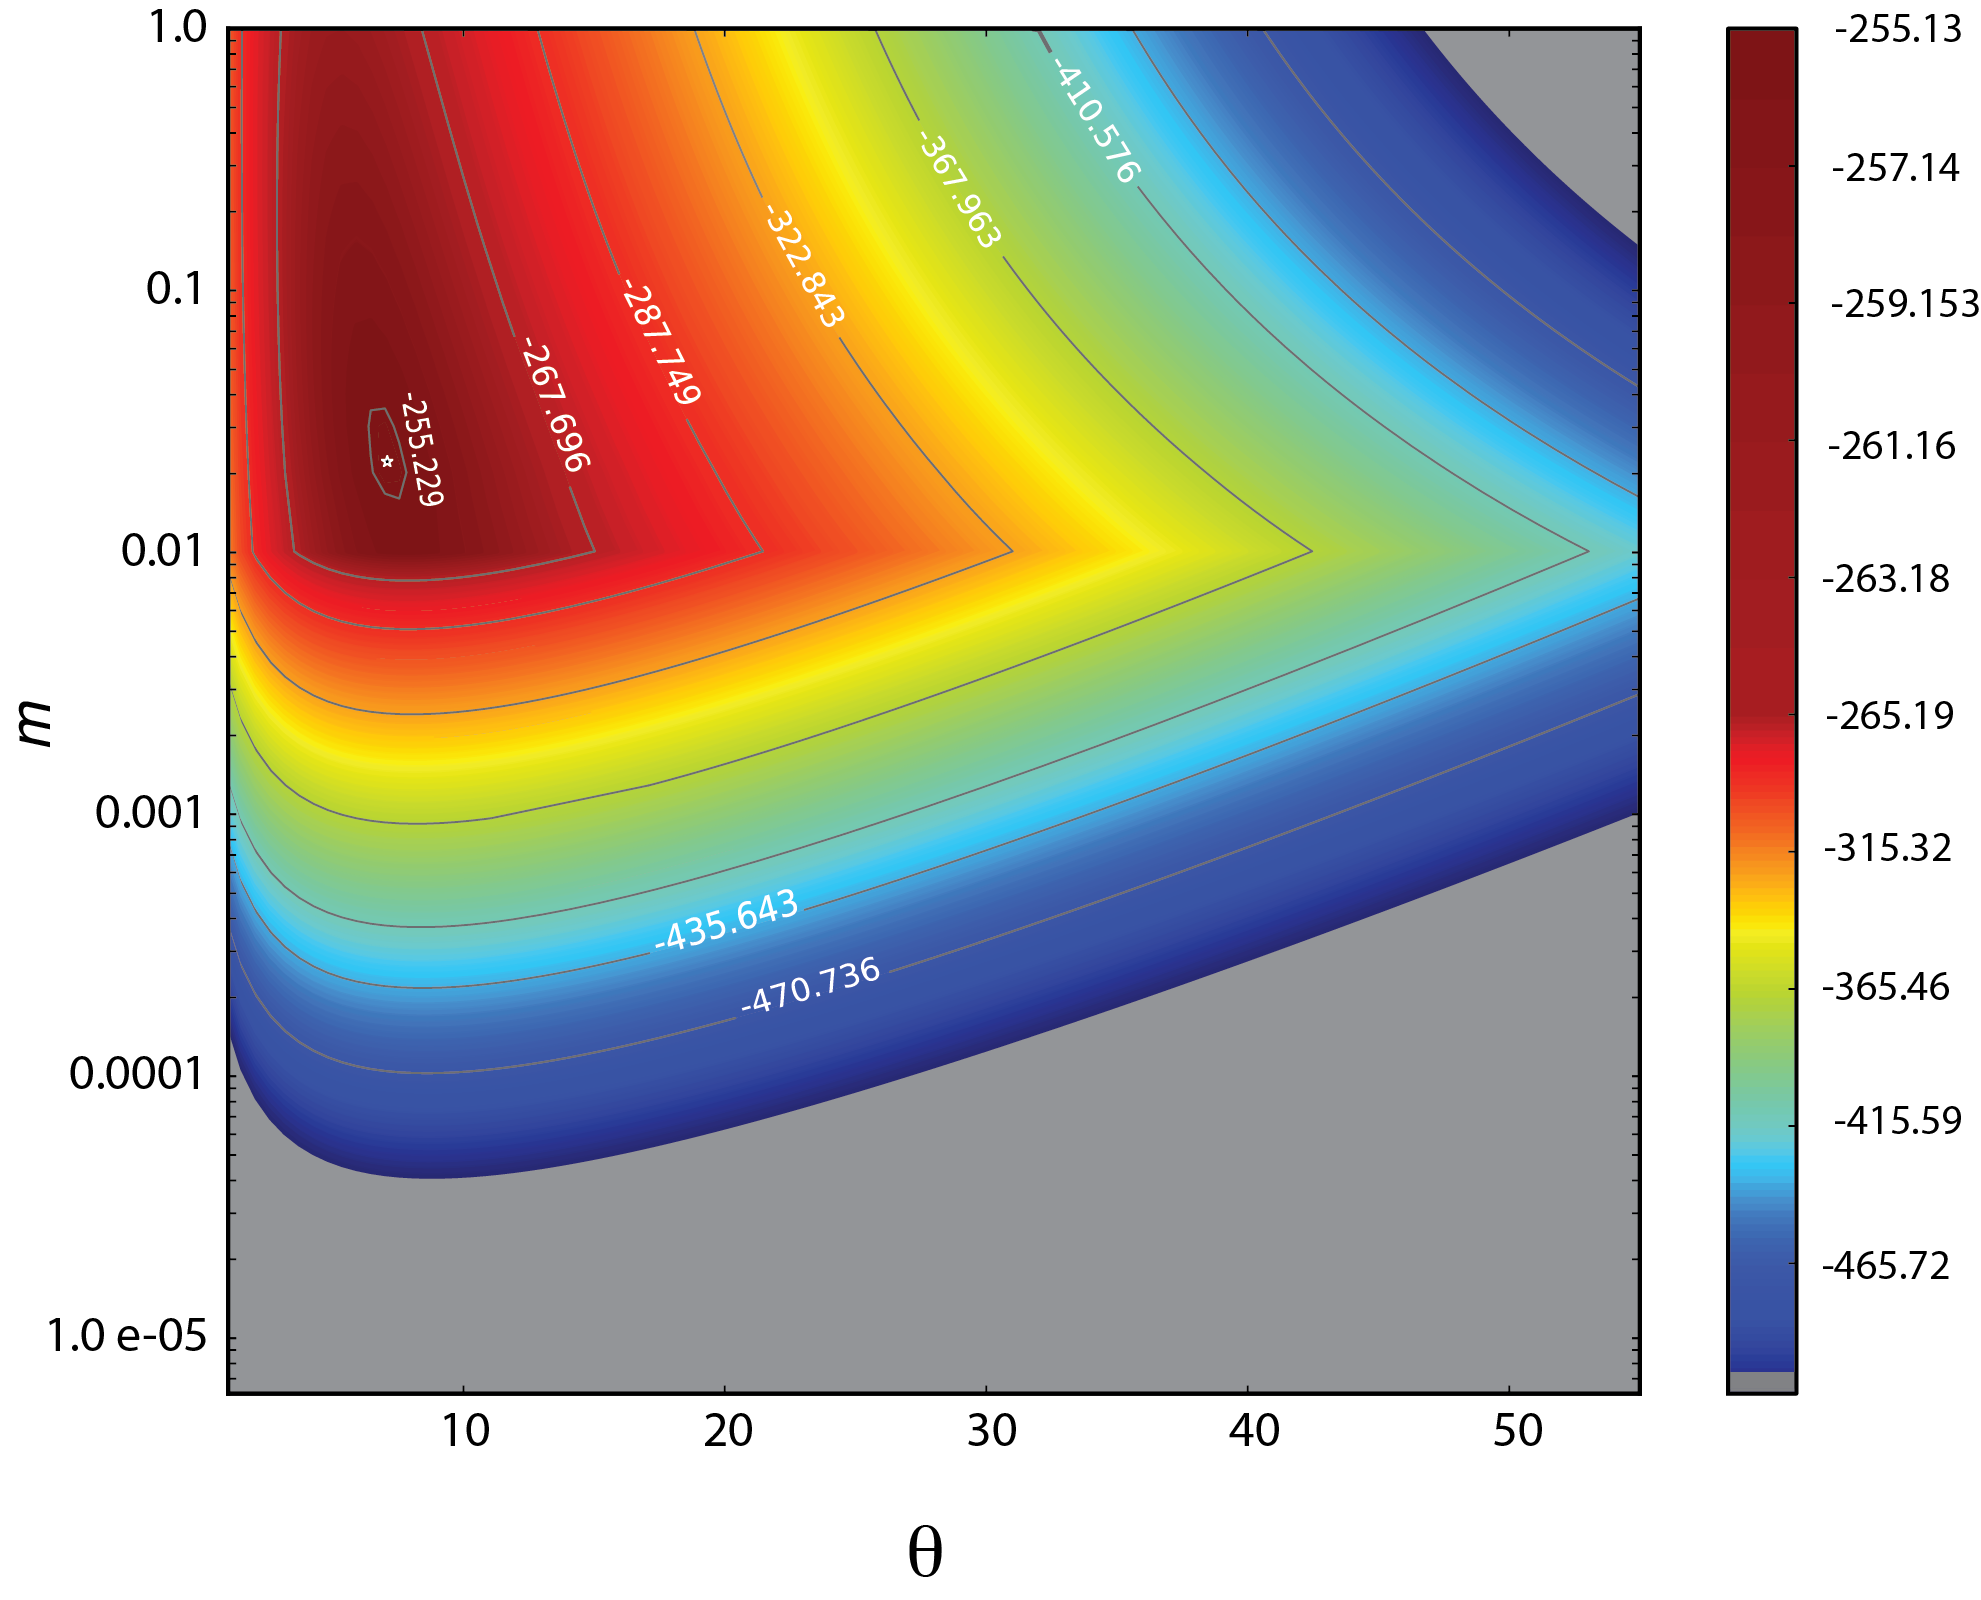
\includegraphics[width=\textwidth]{tex_source/figures/untb_genomes/lnl_chrom.png}
\caption[Maximum likelihood inference of neutral parameters.]{{\bf Maximum likelihood inference of neutral parameters.}\\ Log likelihood surface as a function of migration rate ($m$), and the fundamental biodiversity number ($\theta$) for \textit{D. rerio} chromosome 19. Dark red color shows regions of the surface where parameters maximize the probability to explain abundances and diversity of genetic elements in the chromosome. Likelihood ratio tests favored Etienne in contrast to Ewens sampling formula to explain the observed data in the chromosome.}
\label{fig:lnl_chrom}
\end{figure}

\subsection{Model testing}

In order to compare and test the fit of the two models computed, a likelihood ratio test \cite{Wilks1938} was conducted thanks to the fact that Etienne's model is nested into Ewens'. Etienne's model has two free parameters while Ewens' only one (under this model $m$ parameter is fixed to 1), thus the number of degrees of freedom for the chi-squared distribution is 1.

Additionally, given the large number of test performed, statistical significances were corrected by false discovery rate (FDR) \cite{Benjamini2001}. Etienne's model was thus kept as best fit model for only those chromosomes that pass the LRT after FDR adjustment, otherwise the null model using Ewens' formula was selected.

\subsection{Test for neutrality}

In the last years two exact tests were developed in order to accept or reject the neutrality of a given community. Both tests are based on the comparison of a given number of random neutral community generated using the parameters estimated (see \ref{sec:model-optimization}) for the real data under neutrality. The comparison of the random neutral communities with the observed distribution of abundances, is the key point to test for neutrality.

The first of these tests \cite{Etienne2007} consists in comparing the distribution of likelihoods of fitting neutral model. This corresponding distribution of random neutral abundances is compared to the likelihood of the observed data. The major problem of this test is technical, the computation time needed to optimize the parameters of each abundance distribution and get the likelihoods is unrealistically too high when dealing with genomic elements.

The second test \cite{Jabot2011} uses, instead of likelihood, the comparison of Shannon's entropy \cite{Shannon1948}, and is much faster as random neutral abundances do not need to be fitted into a neutral model.

Thus, from the neutral parameters obtained for each chromosome, we simulated 10,000 distributions of abundances of genetic elements and computed, for each,  its Shannon's entropy ($H$). Chromosomes were considered significantly non-neutral when the $H$ of their abundances was below 95\% of the 10,000 random neutral values. As an example \fref{fig:shannon_distrib}{}, shows the distribution of H for 10,000 random neutral abundance generated under Etienne's model with $S$, $J$ fixed to the observed numbers and $\theta$ and $m$ corresponding to optimized values for \textit{Anopheles gambiae's} chromosome 2L. In this figure the empirical value of H is below the 95\% of the random neutral distribution, than this chromosome is considered to be non-neutral.

Again, given the high number of tests performed, all p-values obtained from this test were corrected by FDR.

\begin{figure}[htpb]
\centering 
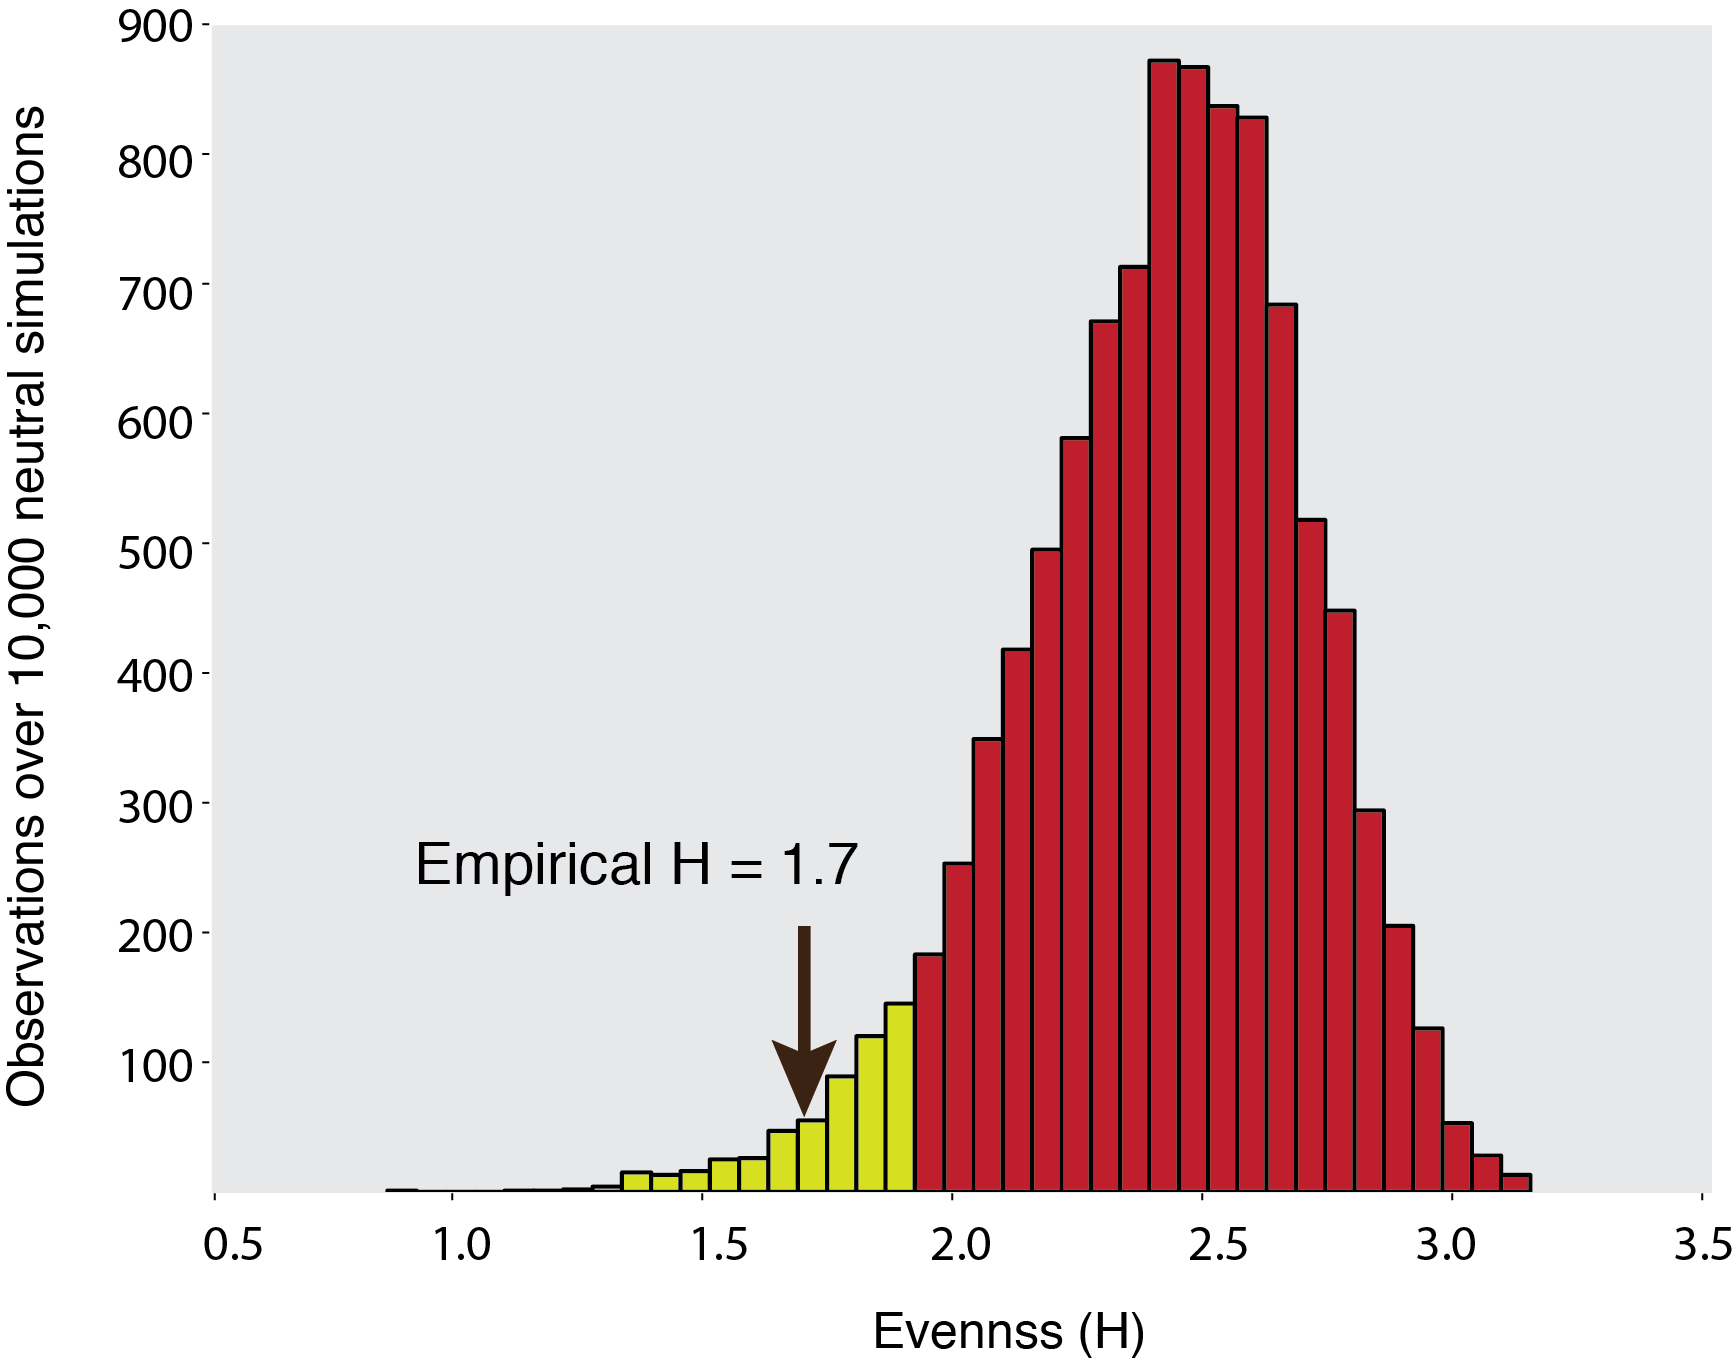
\includegraphics[width=\textwidth]{tex_source/figures/untb_genomes/shannon_distrib.png}
\caption[Comparing simulated and empirical evenness.]{{\bf Comparing simulated and empirical evenness. }\\Neutrality test statistically compares simulated null distribution of H with the empirical H value of the corresponding chromosome. In this case, the null distribution of H values was derived from 10,000 neutral simulations of A. gambiae chromosome 2L, with neutral parameters ($\theta$ and $m$) optimized by ML using Etienne sampling formula. Yellow and red bars display 5\% and 95\% of the simulated neutral data, respectively. Although in this case neutrality was rejected (p= 0.01), posterior correction by multiple testing favored the null neutral hypothesis (q= 0.21).}
\label{fig:shannon_distrib}
\end{figure}



%%% Local Variables: 
%%% mode: latex
%%% TeX-master: "../../master"
%%% End: 
